\documentclass[tikz,border=10pt,multi=tikzpicture]{standalone}
\usepackage{amsmath}
\usepackage{xcolor}
\usetikzlibrary{calc}
\definecolor{mainblue}{HTML}{001158}
\definecolor{accent}{HTML}{8592bc}
\definecolor{lightaccent}{HTML}{e7e9f2}
\definecolor{normalcolor}{HTML}{2a9d8f}
\definecolor{shearcolor}{HTML}{c1121f}
\definecolor{loadcolor}{HTML}{e67e22}

\begin{document}

% ---------- PAGE 1: coordinate system, deflection curve, curvature ----------
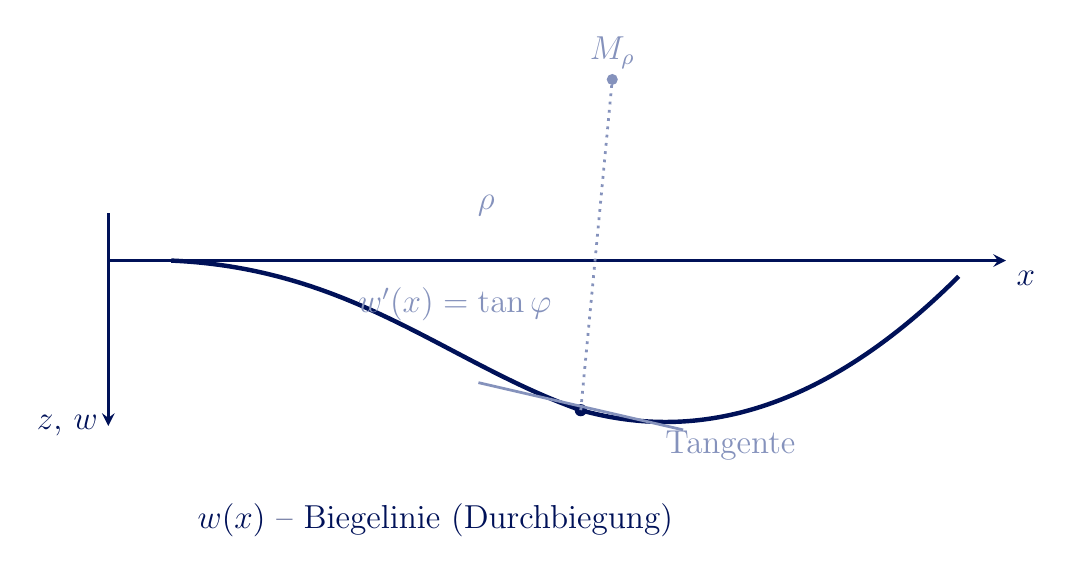
\begin{tikzpicture}[>=stealth, line width=1pt, font=\large]
  % undeformed reference line
  \draw[accent, dashed, line width=0.8pt] (0,0) -- (10,0);

  % deflection curve w(x) (exaggerated)
  \draw[mainblue, line width=1.6pt]
    (0,0) .. controls (2.3,-0.1) and (3.5,-1.3) .. (5.2,-1.9)
          .. controls (7.0,-2.4) and (8.6,-1.6) .. (10,-0.2);

  % x,z axes
  \draw[->, mainblue] (-0.8,0) -- (10.6,0) node[below right] {$x$};
  \draw[->, mainblue] (-0.8,0.6) -- (-0.8,-2.1) node[left] {$z,\,w$};

  % point on curve
  \coordinate (P) at (5.2,-1.9);
  \fill[mainblue] (P) circle (2.2pt);
  \draw[accent, line width=1pt] (3.9,-1.55) -- (6.5,-2.15);
  \node[accent] at (7.1,-2.35) {Tangente};

  % tangent angle
  \node[accent] at (3.6,-0.55) {$w'(x)=\tan\varphi$};

  % radius of curvature sketch (center above the curve, exaggerated)
  \coordinate (M) at (5.6, 2.3);
  \draw[accent, dotted, line width=1pt] (P) -- (M);
  \fill[accent] (M) circle (2pt) node[above] {$M_\rho$};
  \node[accent] at (4.0,0.7) {$\rho$};

  \node[mainblue, anchor=west] at (0.2,-3.3) {$w(x)$ -- Biegelinie (Durchbiegung)};
\end{tikzpicture}

% ---------- PAGE 2: exact curvature geometry (arc ds, d\varphi) ----------
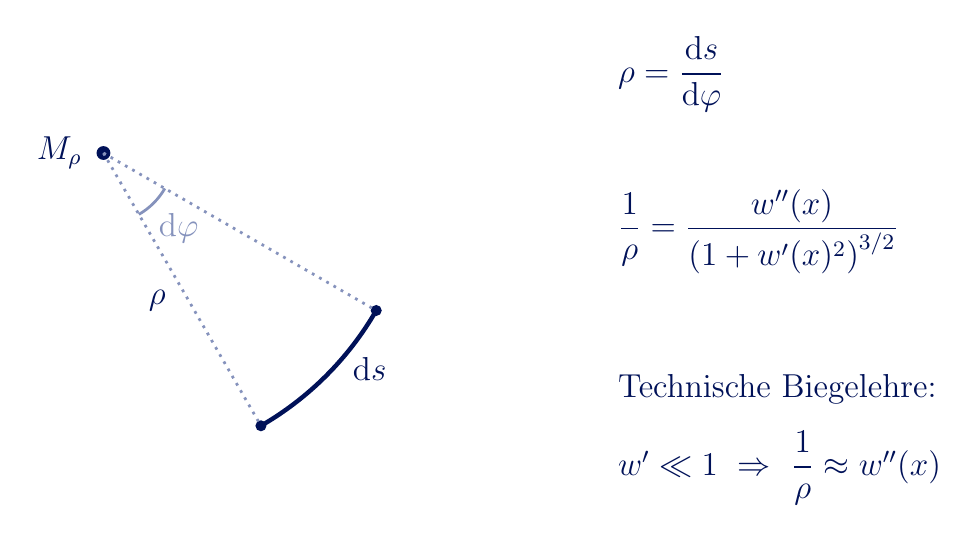
\begin{tikzpicture}[>=stealth, line width=1pt, font=\large]
  \coordinate (M) at (0,0);
  \fill[mainblue] (M) circle (2.5pt) node[left=4pt] {$M_\rho$};

  \draw[mainblue, line width=1.6pt] (-60:4) arc (-60:-30:4);

  \coordinate (A) at (-60:4);
  \coordinate (B) at (-30:4);
  \fill[mainblue] (A) circle (2pt);
  \fill[mainblue] (B) circle (2pt);

  \draw[accent, dotted] (M) -- (A);
  \draw[accent, dotted] (M) -- (B);
  \draw[accent] (-60:0.9) arc (-60:-30:0.9);
  \node[accent] at (-45:1.35) {$\mathrm d\varphi$};

  \node[mainblue] at (-39:4.35) {$\mathrm ds$};
  \node[mainblue] at (-70:2.0) {$\rho$};

  \node[mainblue, font=\large, anchor=west] at (6.4,1.0) {$\rho = \dfrac{\mathrm ds}{\mathrm d\varphi}$};

  \node[mainblue, font=\large, anchor=west] at (6.4,-1.0) {$\dfrac{1}{\rho} = \dfrac{w''(x)}{\left(1+w'(x)^2\right)^{3/2}}$};

  \node[mainblue, font=\large, anchor=west] at (6.4,-3.0) {Technische Biegelehre:};
  \node[mainblue, font=\large, anchor=west] at (6.4,-4.0) {$w' \ll 1 \ \Rightarrow\ \dfrac{1}{\rho}\approx w''(x)$};
\end{tikzpicture}

% ---------- PAGE 3: differential beam element dz (equilibrium) ----------
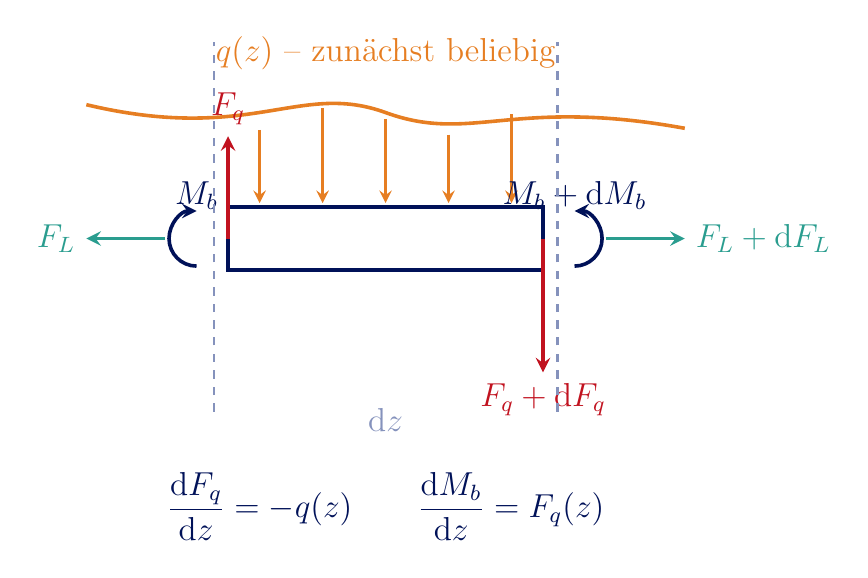
\begin{tikzpicture}[>=stealth, line width=1pt, font=\large]
  % beam element box
  \draw[mainblue, line width=1.4pt] (0,0) rectangle (4,0.8);

  % distributed load q(z): arbitrary, closed-form function above the element
  \draw[loadcolor, line width=1.3pt]
    (-1.8,2.1) .. controls (0.3,1.6) and (0.9,2.4) .. (2.0,2.0)
               .. controls (3.1,1.6) and (3.6,2.2) .. (5.8,1.8);
  \foreach \x/\y in {0.4/1.78, 1.2/2.06, 2.0/1.92, 2.8/1.72, 3.6/1.98} {
    \draw[loadcolor, ->, line width=1pt] (\x,\y) -- (\x,0.85);
  }
  \node[loadcolor] at (2.0,2.75) {$q(z)$ -- zunächst beliebig};

  % left cut face, left to right: F_L (arrow pointing further left), M_b, Balken
  \draw[normalcolor, ->, line width=1.3pt] (-0.8,0.4) -- (-1.8,0.4) node[left] {$F_L$};
  \draw[mainblue, ->, line width=1.3pt] let \p1=($(-0.4,0.4)+(270:0.35)$) in (\p1) arc (270:90:0.35);
  \node[mainblue] at (-0.4,0.95) {$M_b$};
  \draw[shearcolor, ->, line width=1.3pt] (0,0.4) -- (0,1.7) node[above] {$F_q$};

  % right cut face, left to right: Balken, M_b+dM_b, F_L+dF_L (arrow pointing further right)
  \draw[shearcolor, ->, line width=1.3pt] (4,0.4) -- (4,-1.3) node[below] {$F_q+\mathrm dF_q$};
  \draw[mainblue, ->, line width=1.3pt] let \p1=($(4.4,0.4)+(-90:0.35)$) in (\p1) arc (-90:90:0.35);
  \node[mainblue] at (4.4,0.95) {$M_b+\mathrm dM_b$};
  \draw[normalcolor, ->, line width=1.3pt] (4.8,0.4) -- (5.8,0.4) node[right] {$F_L+\mathrm dF_L$};

  \draw[accent, dashed] (-0.18,-1.8) -- (-0.18,2.9);
  \draw[accent, dashed] (4.18,-1.8) -- (4.18,2.9);
  \node[accent] at (2.0,-1.9) {$\mathrm dz$};

  \node[mainblue, font=\large] at (2.0,-3.0) {$\dfrac{\mathrm dF_q}{\mathrm dz} = -q(z) \qquad \dfrac{\mathrm dM_b}{\mathrm dz} = F_q(z)$};
\end{tikzpicture}

\end{document}
